\documentclass[11pt,a4paper]{article}

\usepackage{main}
\usepackage{cours}

\renewcommand{\typedocument}{Document}
\renewcommand{\classe}{5e}
\renewcommand{\titre}{La production d'électricité}

\begin{document}

\partie{Production d’électricité en France et dans le monde en 2024 par sources d’énergie}

\vspace*{-1em}

\begin{center}
    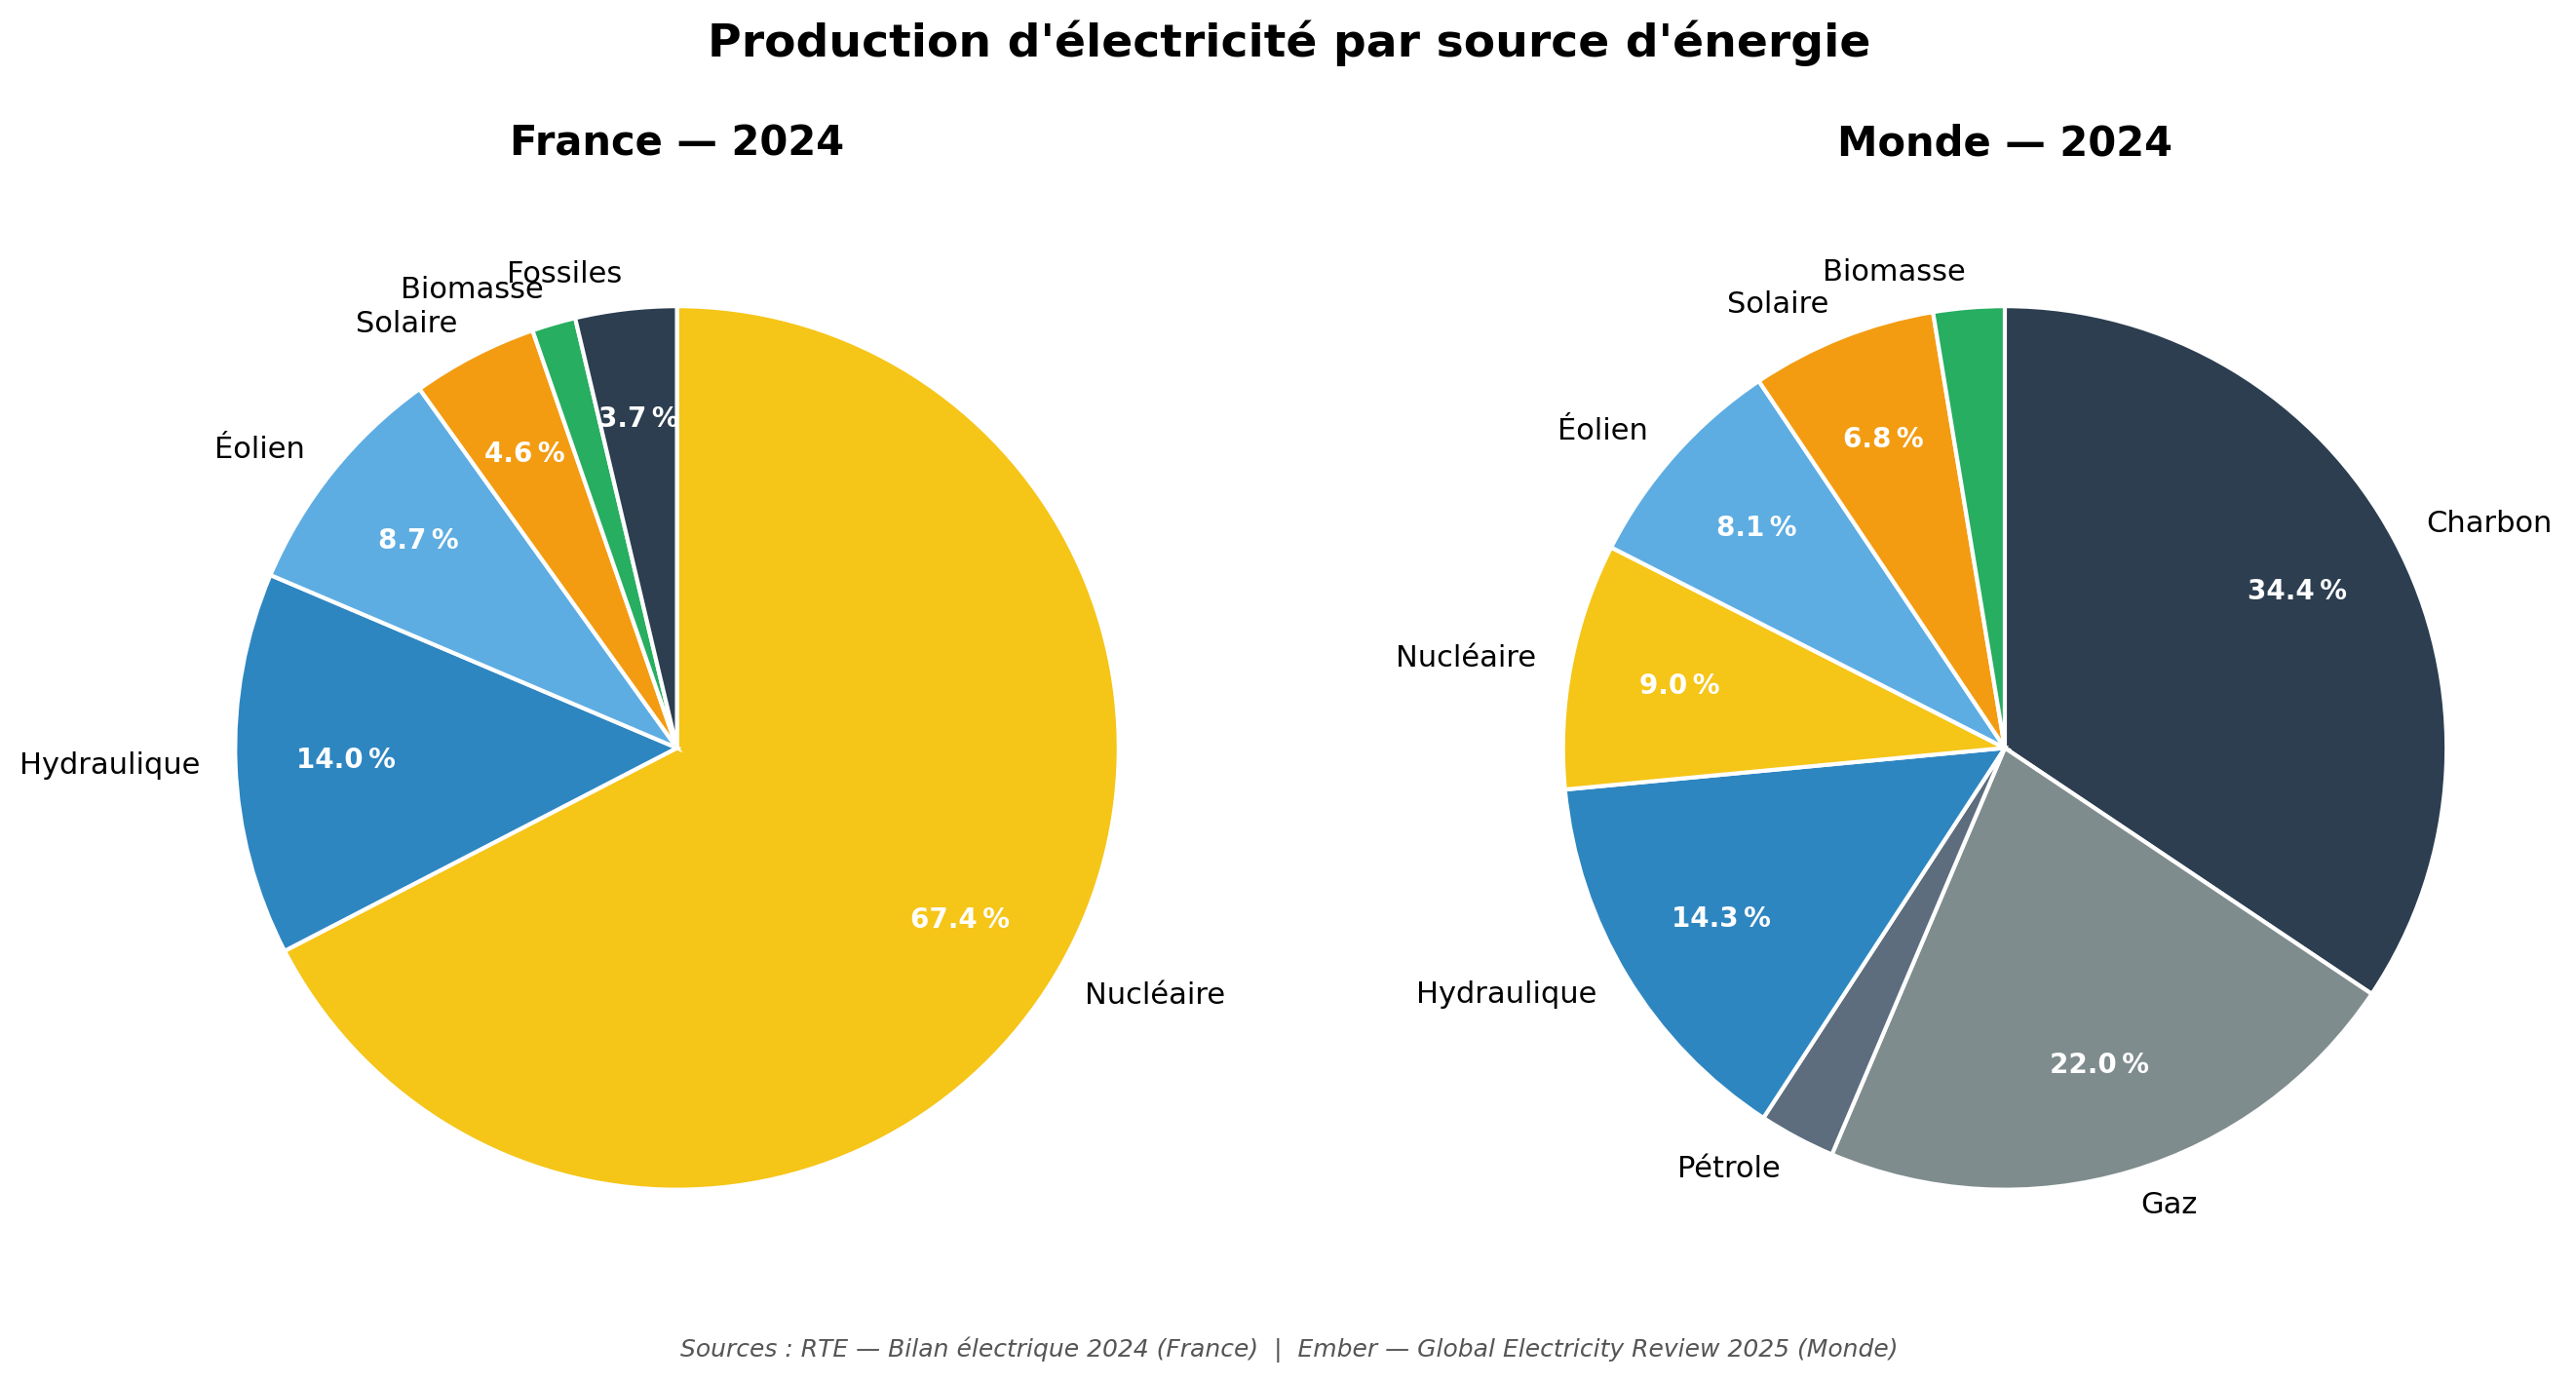
\includegraphics[width=14cm]{images/camemberts_electricite_2024.png}
\end{center}

\vspace*{-1em}

\partie{Les différents moyens de production d'énergie électrique}

L'électricité que nous utilisons à la maison n'existe pas à l'état naturel : il faut la fabriquer. C'est le rôle des centrales électriques.

Dans presque toutes les centrales (à part le panneau solaire), le principe est le même : faire tourner un appareil appelé alternateur. Cet alternateur transforme le mouvement de rotation en électricité.

Certaines sources d'énergies sont dites fossiles : le charbon, le pétrole, le gaz. Quand on les brûle, on rejette dans l'atmosphère un gaz appelé dioxyde de carbone (CO\textsubscript{2}). C'est un gaz à effet de serre : il retient la chaleur du Soleil près de la Terre, ce qui fait augmenter la température moyenne de la planète.

Les conséquences sont la fonte des glaciers, la montée du niveau des mers, des sécheresses…

Les énergies fossiles sont non renouvelables. À force de les consommer, les réserves diminuent. Un jour, il n'y en aura plus.

\important{Focus sur: le panneau solaire}

\begin{center}
    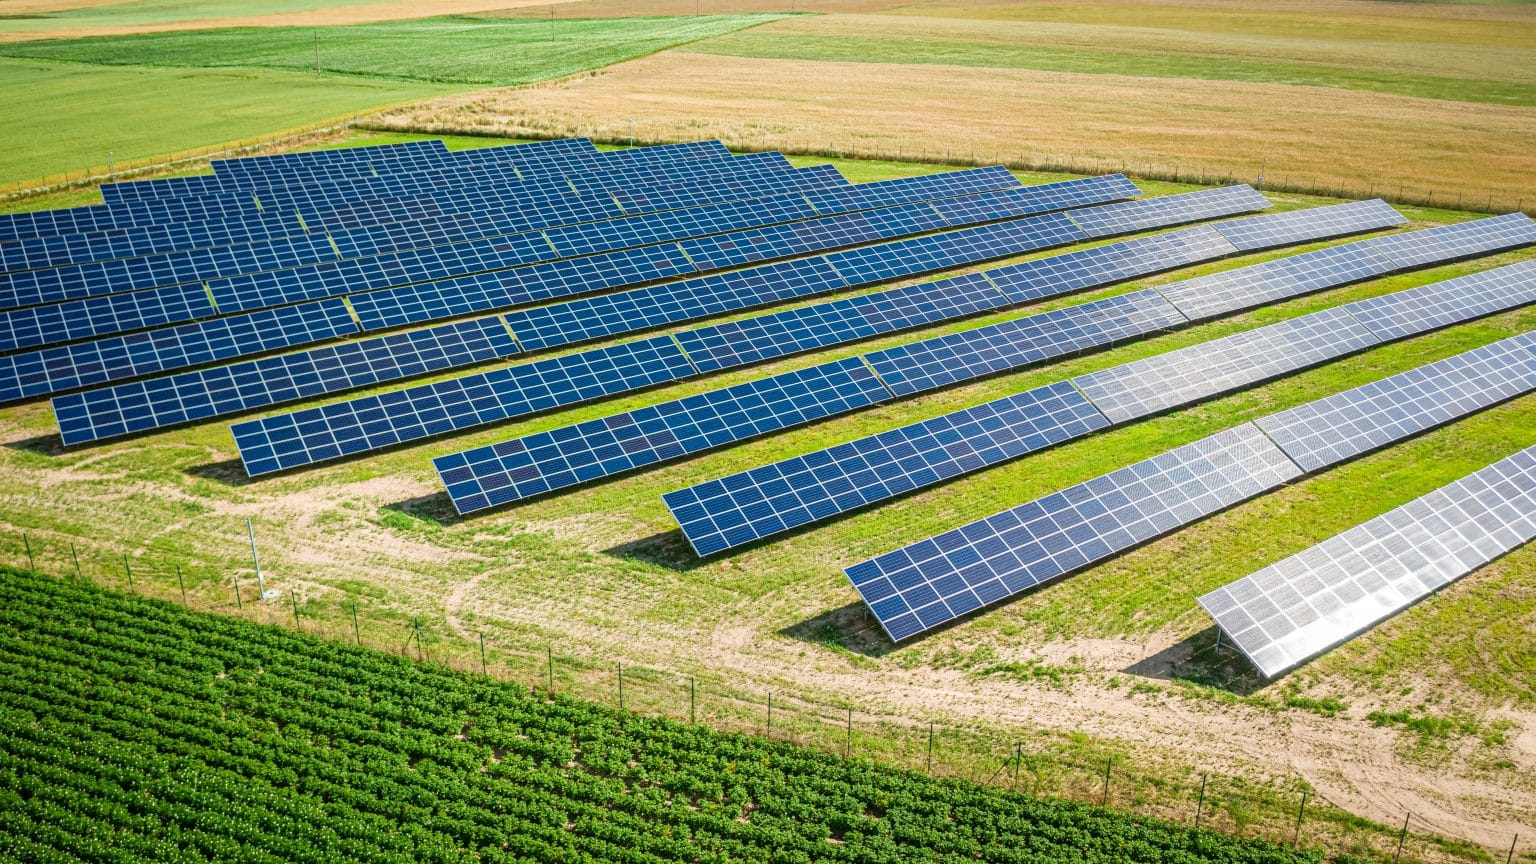
\includegraphics[width=8cm]{images/panneau solaire.jpg}

    \textit{Ferme solaire photovoltaïque}
\end{center}


Un panneau solaire est un dispositif qui permet de produire de l'électricité à partir de la lumière du Soleil. Il est composé de cellules photovoltaïques, le plus souvent de couleur bleu foncé, qui transforment directement la lumière en électricité.
Contrairement aux autres moyens de production, le panneau solaire ne possède pas d'alternateur : il n'y a aucune pièce en mouvement.
Pour produire beaucoup d'électricité, on installe souvent un grand nombre de panneaux sur un même terrain : c'est ce qu'on appelle une ferme solaire ou une centrale solaire.

Le panneau solaire utilise la lumière du Soleil, une source d'énergie renouvelable, et ne rejette pas de CO\textsubscript{2}. La production d'électricité dépend de la météo et du moment de la journée : elle est nulle la nuit et faible quand le ciel est couvert.
Une ferme solaire occupe une grande surface au sol, et la fabrication des panneaux nécessite des matériaux rares.

\end{document}